\documentclass{standalone}
%<--------------------------------------------------------------------------->%
%%% Math %%%
\usepackage{amsmath}
%<--------------------------------------------------------------------------->%
% %%% Hyper Reference %%%
% \usepackage[hidelinks,colorlinks=true]{hyperref}
% %<--------------------------------------------------------------------------->%
%%% TikZ %%%
\usepackage{tikz}
% \usetikzlibrary{calc}
% \usetikzlibrary{angles,quotes}
\usetikzlibrary{intersections,topaths}
% \usetikzlibrary{decorations.markings}
\usetikzlibrary{svg.path}
%<--------------------------------------------------------------------------->%
%% References:
%% https://www.akc.org/expert-advice/health/how-to-calculate-dog-years-to-human-years/

\begin{document}

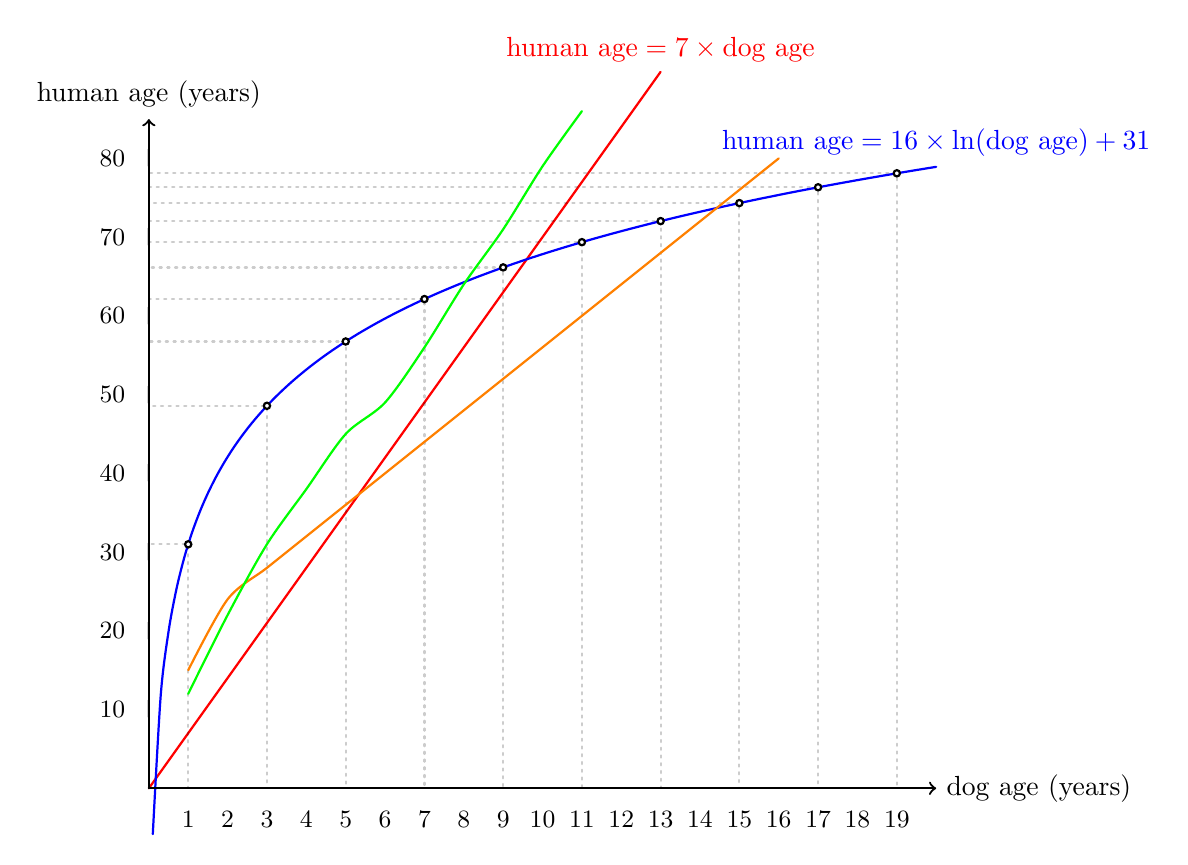
\begin{tikzpicture}[scale=1/10,thick,line cap=round,xscale=5]
	\tikzstyle{jiao}=[solid,circle,draw,fill=white,inner sep=.8pt];
	%% conversion
	\draw[red,smooth,samples=100,domain=0:13]                  plot(\x,{7*\x});
	\draw[name path=LOG,blue,smooth,samples=100,domain=0.1:20] plot(\x,{16*ln((\x))+31});
	%% correspondence
	\draw[name path=A,draw=none] (1,0)  -- +(0,80);
	\draw[name path=B,draw=none] (3,0)  -- +(0,80);
	\draw[name path=C,draw=none] (5,0)  -- +(0,80);
	\draw[name path=D,draw=none] (7,0)  -- +(0,80);
	\draw[name path=E,draw=none] (9,0)  -- +(0,80);
	\draw[name path=F,draw=none] (11,0) -- +(0,80);
	\draw[name path=G,draw=none] (13,0) -- +(0,80);
	\draw[name path=H,draw=none] (15,0) -- +(0,80);
	\draw[name path=I,draw=none] (17,0) -- +(0,80);
	\draw[name path=J,draw=none] (19,0) -- +(0,80);
	\path[name intersections={of=LOG and A}]; \draw[dotted,draw=black,opacity=0.2] (0,0) -| (intersection-1) node[jiao,opacity=1]{} -| (0,0);
	\path[name intersections={of=LOG and B}]; \draw[dotted,draw=black,opacity=0.2] (0,0) -| (intersection-1) node[jiao,opacity=1]{} -| (0,0);
	\path[name intersections={of=LOG and C}]; \draw[dotted,draw=black,opacity=0.2] (0,0) -| (intersection-1) node[jiao,opacity=1]{} -| (0,0);
	\path[name intersections={of=LOG and D}]; \draw[dotted,draw=black,opacity=0.2] (0,0) -| (intersection-1) node[jiao,opacity=1]{} -| (0,0);
	\path[name intersections={of=LOG and E}]; \draw[dotted,draw=black,opacity=0.2] (0,0) -| (intersection-1) node[jiao,opacity=1]{} -| (0,0);
	\path[name intersections={of=LOG and F}]; \draw[dotted,draw=black,opacity=0.2] (0,0) -| (intersection-1) node[jiao,opacity=1]{} -| (0,0);
	\path[name intersections={of=LOG and G}]; \draw[dotted,draw=black,opacity=0.2] (0,0) -| (intersection-1) node[jiao,opacity=1]{} -| (0,0);
	\path[name intersections={of=LOG and H}]; \draw[dotted,draw=black,opacity=0.2] (0,0) -| (intersection-1) node[jiao,opacity=1]{} -| (0,0);
	\path[name intersections={of=LOG and I}]; \draw[dotted,draw=black,opacity=0.2] (0,0) -| (intersection-1) node[jiao,opacity=1]{} -| (0,0);
	\path[name intersections={of=LOG and J}]; \draw[dotted,draw=black,opacity=0.2] (0,0) -| (intersection-1) node[jiao,opacity=1]{} -| (0,0);
	%% small dogs
	\draw[orange] plot [smooth] coordinates {(1,15) (2,24) (3,28) (4,32) (5,36) (6,40) (7,44) (8,48) (9,52) (10,56) (11,60) (12,64) (13,68) (14,72) (15,76) (16,80)};
	\draw[green]  plot [smooth] coordinates {(1,12) (2,22) (3,31) (4,38) (5,45) (6,49) (7,56) (8,64) (9,71) (10,79) (11,86) };
	%% axis
	\draw[<->] (0,85) node[above]{human age (years)} -- (0,0) -- (20,0) node[right]{dog age (years)};
	%% human years
	\node[label=above:\small 10,rotate=90] at (0,10) {\tiny |};
	\node[label=above:\small 20,rotate=90] at (0,20) {\tiny |};
	\node[label=above:\small 30,rotate=90] at (0,30) {\tiny |};
	\node[label=above:\small 40,rotate=90] at (0,40) {\tiny |};
	\node[label=above:\small 50,rotate=90] at (0,50) {\tiny |};
	\node[label=above:\small 60,rotate=90] at (0,60) {\tiny |};
	\node[label=above:\small 70,rotate=90] at (0,70) {\tiny |};
	\node[label=above:\small 80,rotate=90] at (0,80) {\tiny |};
	%% dog years
	\node[label=below:\small 1]  at (1,0)  {\tiny |};
	\node[label=below:\small 2]  at (2,0)  {\tiny |};
	\node[label=below:\small 3]  at (3,0)  {\tiny |};
	\node[label=below:\small 4]  at (4,0)  {\tiny |};
	\node[label=below:\small 5]  at (5,0)  {\tiny |};
	\node[label=below:\small 6]  at (6,0)  {\tiny |};
	\node[label=below:\small 7]  at (7,0)  {\tiny |};
	\node[label=below:\small 8]  at (8,0)  {\tiny |};
	\node[label=below:\small 9]  at (9,0)  {\tiny |};
	\node[label=below:\small 10] at (10,0) {\tiny |};
	\node[label=below:\small 11] at (11,0) {\tiny |};
	\node[label=below:\small 12] at (12,0) {\tiny |};
	\node[label=below:\small 13] at (13,0) {\tiny |};
	\node[label=below:\small 14] at (14,0) {\tiny |};
	\node[label=below:\small 15] at (15,0) {\tiny |};
	\node[label=below:\small 16] at (16,0) {\tiny |};
	\node[label=below:\small 17] at (17,0) {\tiny |};
	\node[label=below:\small 18] at (18,0) {\tiny |};
	\node[label=below:\small 19] at (19,0) {\tiny |};
	%% equations
	\node[red,above] at (13,13*7) {$\text{human age}=7\times\text{dog age}$};
	\node[blue,above,align=center] at (20,{16*ln(20)+31}) {$\text{human age}=16\times\ln(\text{dog age})+31$};
	% %% title
	% \node[yshift=-1.5cm,align=center] at (10,0) {\Large How old is a dog? (Based on Labrador Retrievers)\\\normalsize\url{https://doi.org/10.1101/829192}};
\end{tikzpicture}

\end{document}
